\def\micro{\mu m}
\def\um{$\micro$ }
\def\degreesC{$\degree C$ }
\def\percent{$\%$ }
\documentclass[10pt,a4paper,oneside]{article}
\usepackage[left=2cm,right=2cm,top=2cm,bottom=2cm]{geometry}

\usepackage[dvipsnames]{xcolor}

%%  -------------------------------------------------------------------
%%      GDS II layer, regarding MOSIS SCMOS layer map
%%  -------------------------------------------------------------------
% GDS II #41 - P_WELL
\definecolor{pwell}{rgb}{1.0, 0.74, 0.53}   % macaroni and cheese
% GDS II #42 - N_WELL
\definecolor{nwell}{rgb}{0.61, 0.87, 1.0}  % columbia blue
\definecolor{pbase}{rgb}{1.0, 0.51, 0.26}  % mango tango
\definecolor{nbase}{rgb}{0.0, 0.75, 1.0}   % capri 
% GDS II #43 - ACITVE
\definecolor{active}{rgb}{0.9, 0.4, 0.38}   % light carmine pink
% GDS II #45 - N_PLUS_SELECT
\definecolor{nimplant}{rgb}{0.45, 0.76, 0.983}% maya blue
% GDS II #44 - P_PLUS_SELECT
\definecolor{pimplant}{rgb}{1.0, 0.51, 0.26}% mango tango
% GDS II #46 - POLY
\definecolor{poly}{rgb}{0.56, 0.93, 0.56}   % light green
% GDS II #25 - CONTACT
\definecolor{contact}{rgb}{0.83, 0.83, 0.83}% light gray
% GDS II #49 - METAL1
\definecolor{metal1}{rgb}{0.38, 0.31, 0.86} % majorelle blue
% GDS II #50 - VIA1
\definecolor{via1}{rgb}{0.83, 0.83, 0.83}   % light gray
% GDS II #51 - METAL2
\definecolor{metal2}{rgb}{0.04, 0.85, 0.32} % malachite
% GDS II #61 - VIA2
\definecolor{via2}{rgb}{0.83, 0.83, 0.83}   % light gray
% GDS II #63 - METAL3
\definecolor{metal3}{rgb}{0.98, 0.93, 0.37} % maize
% GDS II #30 - VIA3
\definecolor{via3}{rgb}{0.83, 0.83, 0.83}   % light gray
% GDS II #31 - METAL4
\definecolor{metal4}{rgb}{0.75, 0.25, 0.0}  % mahogany
% GDS II #32 - VIA4
\definecolor{via4}{rgb}{0.83, 0.83, 0.83}   % light gray
% GDS II #33 - METAL5
\definecolor{metal5}{rgb}{0.79, 0.08, 0.48} % magenta (dye)
% GDS II #36 - VIA5
\definecolor{via5}{rgb}{0.83, 0.83, 0.83}   % light gray
% GDS II #37 - METAL6
\definecolor{metal6}{rgb}{0.11, 0.35, 0.02} % lincoln green
% GDS II #29 - SILICIDE_BLOCK
\definecolor{silicide-block}{rgb}{0.98, 0.94, 0.9}  % linen
% GDS II #52 - GLASS
\definecolor{glass}{rgb}{1.0, 1.0, 0.88}    % light yellow
% GDS II #26 - PADS
\definecolor{pads}{rgb}{0.75, 1.0, 0.0}     % lime (color wheel)

\definecolor{resist}{rgb}{0.71, 0.4, 0.11}  % light brown

\definecolor{silicide}{rgb}{0.29, 0.33, 0.13}
\definecolor{titanium}{rgb}{0.8, 0.58, 0.46}

\def\OpacityLayout {0.5}

%
% physical
%
\definecolor{substrate}{rgb}{0.96, 0.94, 0.93}  % isabelline
\definecolor{nitride}{rgb}{1.0, 0.03, 0.0}
\definecolor{gateoxide}{rgb}{0.88, 1.0, 1.0}    % light cyan
\definecolor{isolationoxide}{rgb}{0.84, 0.79, 0.87}% languid lavender

\usepackage[utf8]{inputenc}
\usepackage[english]{babel}
\usepackage{forloop}
\usepackage{amsmath}
\usepackage{amsfonts}
\usepackage{amssymb}
\usepackage{gensymb}
\usepackage{mdframed}
\usepackage{graphicx}
\usepackage{tikz}
\usetikzlibrary{arrows,automata,shapes}
\usepackage[siunitx]{circuitikz}
\usepackage{makecell}
\usepackage{array}

\def\WaferClean{
\begin{tikzpicture}\node [fill=cyan, rounded corners=5pt] {Clean};\end{tikzpicture}}
\def\WaferSemiClean{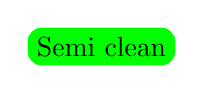
\begin{tikzpicture}\node [fill=green, rounded corners=5pt] {Semi clean};\end{tikzpicture}}
\def\WaferNonStandard{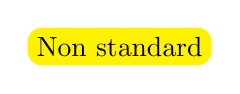
\begin{tikzpicture}\node [fill=yellow, rounded corners=5pt] {Non standard};\end{tikzpicture}}

\usepackage[colorlinks=true,linkcolor=blue,urlcolor=black,bookmarksopen=true]{hyperref}
\usepackage{bookmark}
\usepackage{hyperref}
\usepackage{sepfootnotes}
\usepackage{lipsum,tocloft} 
\usetikzlibrary{positioning}
\usetikzlibrary{patterns}

\usepackage[digital,srcmeas]{circdia}

\usepackage{float}
\floatstyle{boxed} 
\restylefloat{figure}

\title{Libre Silicon process specification}
\date{\today}
\author{David Lanzendörfer}
\makeindex

\newcounter{ct}
\def\CrossSectionOnly{0.3}
\def\CrossAndTopSection{0.2}
\def\CrossAndTopSectionBig{0.3}
\def\VLSILayout{0.4}

\DeclareMathOperator\erfc{erfc}

\setlength{\parindent}{0pt} % get rid of annoying indents

%\numberline{\thefootnotes}
%%#1

%\newcommand{\listfootnotesname}{\section{List of Footnotes}}% 'List of Footnotes' title 
%\newlistof[chapter]{footnotes}{fnt}{\listfootnotesname}% New 'List of...' for footnotes 
%\let\oldfootnote\footnote % Save the old \footnote{...} command 
%\renewcommand\footnote[1]{% Redefine the new footnote to also add 'List of Footnote' entries. 
%	\refstepcounter{footnotes}% Add and step a reference to the footnote/counter. 
%	\oldfootnote{#1}% Make a regular footnote
%	\addcontentsline{fnt}{footnotes}{
%		\protect
%		\tiny{
%			#1
%			%\thefootnotes
%		}
%	}% Add the 'List of...' entry. 
%}

\begin{document}
\maketitle
\begin{abstract}
	Copyright © 2017 LANCEVILLE TECHNOLOGY GROUP CO., LIMITED. All rights reserved. \\

	This process is licensed under the Libre Silicon public license; you can redistribute it and/or modify it under the terms of the Libre Silicon public license
	as published by the Libre Silicon alliance, either version 1 of the License, or (at your option) any later version.

	This design is distributed in the hope that it will be useful, but WITHOUT ANY WARRANTY; without even the implied warranty of MERCHANTABILITY or FITNESS FOR A PARTICULAR PURPOSE.
	See the Libre Silicon Public License for more details. \\

	This document is part of the specification of the free silicon manufacturing standard for manufacturing the LibreSilicon standard logic cells\footnote{\url{https://github.com/chipforge/StdCellLib}} and related free technology nodes from the LibreSilicon project.

	For this initial revision 0.1 a gate-first approach has been chosen which led to the choice of polysilicon as the gate electrode material because of the simplicity of the gate alignment.
	For better isolation properties of the transistors and gates in overall a box-isolation approach has been chosen.
	All of these choices have been made with the future scale down from the recent $1 \mu m$ to smaller structure sizes.
	\textbf{This process is for manufacturing $1 \mu m$ only!}
	But further releases which will have been tested with smaller structure sizes can be expected.
\end{abstract}
\newpage

We need to optimize our process to be TTL compatible (5V logic levels) and at the same time being as fast and power efficient as possible.
In order to have a good propagation delay with a technology node of around $1\mu m$ we will have to have gates with up to four stacked MOS transistors.

Acceptable input signal voltages range from 0 volts to 0.8 volts for a low logic state, and 2 volts to 5 volts for a high logic state.
Acceptable output signal voltages shall range from 0 volts to 0.5 volts for a low logic state, and 2.7 volts to 5 volts for a high logic state\footnote{\url{https://www.allaboutcircuits.com/textbook/digital/chpt-3/logic-signal-voltage-levels}}

\begin{figure}[H]
	\centering
	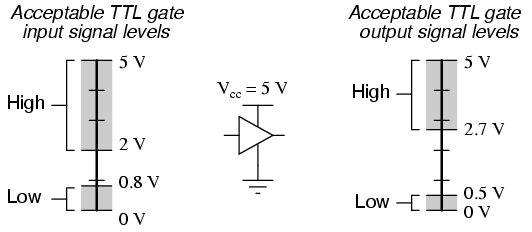
\includegraphics[scale=0.5]{logic_levels.png}
	\caption{TTL logic levels}
	\label{TTL_logic_levels}
\end{figure}

As shown in \autoref{TTL_logic_levels} we have some margin to make our PMOS and NMOS transistors work with each other in order to form a CMOS circuit which is actually working without getting warm.

Or more clearly defined
\begin{equation}
V_{off} \leq 0.8V
\end{equation}
and
\begin{equation}
V_{on} \geq 2V
\end{equation}
which are limits, elementary to our design.

\begin{figure}[H]
	\centering
	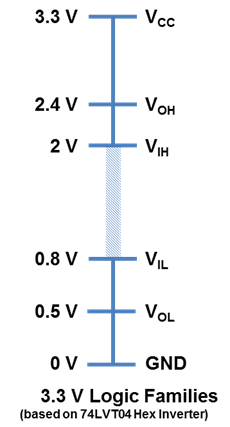
\includegraphics[scale=0.5]{cmos_3v3.png}
	\caption{CMOS 3.3V logic levels}
	\label{CMOS_logic_levels}
\end{figure}

This means that we also will be compatible to CMOS logic level output pins since their ON/OFF levels are within our tolerance range\footnote{\url{https://learn.sparkfun.com/tutorials/logic-levels/33-v-cmos-logic-levels}} as it is shown in \autoref{CMOS_logic_levels}.

We target threshold voltages of $V_{Tn} \approx 0.8V$ and $V_{Tp} \approx -0.8V$ which should be enough.
We can internally always shift the voltage supply levels to compensate for threshold variations.\footnote{Hagen! Please explain this part here}
\newpage
\input{process_design_requirements.tex}
\subsection{Substrate}
For this process p-substrate is being used, but forks and modifications will be very well possible based on a Graphene substrate or alike, still under the LSPL.
The starting material is a p-type, <100> oriented silicon with a doping concentration of $\approx 9\times10^{14}cm^{-3}$.\\

\textbf{Reasons for using p-substrate}:\begin{itemize}
\item We can't use two different substrates for our design because in the design both PMOS and NMOS is present.
We have to choose which is more beneficial from fabrication point of view.
In general or say it's true that NMOS devices are always more in the Semiconductor Industry in comparison to PMOS devices.
For your reference-SRAM requires 6 transistors (4 NMOS, 2 PMOS).
\item Another reason for more number of NMOS is because of difference of mobility of electron and holes.
Electron mobility is almost twice of holes mobility and because of this ON-RESISTANCE of n-channel device is half of p-channel device with the same geometry and under the same operating conditions.
That means to achieve same impedance size of n-channel transistors is almost half of p-channel devices.
Same thing I can say in the different way that for same size of wafer, we can have more number of NMOS (means can perform more logical operation) in comparison to PMOS.
\end{itemize}
\subsection{Isolation}
For the isolation (\autoref{sti})  in this design the STI approach is being chosen.
Shallow trench isolation (STI), also known as box isolation technique, is an integrated circuit feature which prevents electric current leakage between adjacent semiconductor device components.\footnote{\url{https://www.google.com/patents/US7985656}}
STI is generally used on CMOS process technology nodes of 250 nanometers and smaller.\\

\textbf{Reasons for using box isolation}:\begin{itemize}
\item We want to be forward compatible to future LibreSilicon nodes with a size of 100nm or smaller
\item It simplifies the construction of the gate and allows us to use Aluminum instead of Polysilicon for the gate contact
\end{itemize}

\subsection{Interconnect}
The interconnects and the gate electrode are being made using Aluminum which is a very commonly used material to do interconnects in low-frequency and low-resolution applications \\

\textbf{Reasons for using Aluminum}:\begin{itemize}
\item It's a well explored material for interconnect with a lot of literature on how to process it
\item Aluminum is easy to etch compared to copper
\item It isn't contaminating everything like copper does and doesn't require special separated setup for handling
\item The machines at HKUST can do CMP for copper only on 4 inch wafers which would limit us in wafer size
\end{itemize}

\begin{mdframed}[linewidth=2pt,linecolor=green]
As soon as we've got CMOS all figured out, we will tackle copper interconnect in release 2.0
\end{mdframed}
\newpage
\section{MOS gate material}
We decided to use the gate-first approach because realizing the gate self-alignment is much easier this way.
We further on decided to use the best-practice material polysilicon for the gate electrode, because it is easy to deposit and etch and virtually every manufacturer out there has at least one machine in their lab to deposit it.
Because of its high resistance however, we had to throw in another layer of silicide in order to reduce the gate resistivity from these $100 \Omega-m$ or so to a a few Ohms per meter.
A nice side effect is the better etch-stop properties of this low-resistance film adding to the gate, source and drain contacts.

A down side is that we will have to get "a hang on" the reaction times of silicides because a lot of the details of the reactivity between silicon and titanium to form titanium-silicide seem to be under NDA and secrets of the diverse factories running their own CMOS processes.

\section{MOS gate thickness}\label{gate_dimensioning}
As the continuous down-scaling of the device size has lead to very thin gate oxides, the leakage current that can flow from the channel to the gate comes into the order of the subthreshold leakage current and the gate cannot be considered as an ideally insulated electrode anymore.
This affects the circuit functionality and increases the standby power consumption due to the static gate current.
For dynamic logic concepts the gate leakage drastically reduces the maximum clock cycle time\footnote{N. Wang, Digital MOS Integrated Circuits, Prentice-Hall, Englewood Cliffs, NJ, 1989}.
Two tunneling mechanisms are responsible for the gate leakage, Fowler-Nordheim tunneling and direct tunneling\footnote{A. Schenk and G. Heiser, "Modeling and Simulation of Tunneling through Ultra-Thin Gate Dielectrics"J.Appl.Phys., vol. 81, no. 12, pp. 7900, 1997}.
The gate leakage increases exponentially as the oxide thickness is reduced.
This limits the down-scaling of the oxide thickness to about 1.5-2 nm when looking at the total standby power consumption of a chip\footnote{Y. Taur, "The Incredible Shrinking Transistor," IEEE Spectrum, pp. 25-29, July 1999.}.
To further decrease the effective oxide thickness alternative high dielectric constant materials can be used\footnote{S. Thompson, P. Packan, and M. Bohr, "MOS Scaling: Transistor Challenges for the 21st Century," Intel Technology Journal, vol. Q3, 1998}.
On the other hand, a thin gate oxide reduces the short-channel effect and improves the driving capabilities of a MOS transistor.
However, a tradeoff between this benefit and the gate leakage is necessary.\\

With $1 \mu m$ we don't have to worry about this leakage yet because our gate oxide thickness is too high for these effects to actually become a problem, but we want to do our home work already in preparation of scale-down and also for curiosity.

We for now just use 40 nm. That's still doable with a precision high enough when using dry oxidation and a temperature of 1000\degree Celsius.

\subsection{Subthreshold leakage}\label{sub_threshold_leakage}

The sub-threshold leakage current can be calculated with\footnote{\url{http://ecee.colorado.edu/\~bart/book/book/chapter3/ch3_4.htm\#3_4_2}}
\begin{equation}
I_{sub}
=
I_0
\cdot
\left(1-\exp\left(-\frac{V_{ds}}{V_{th}}\right)\right)
\cdot
\exp\left(\frac{V_{gs}-V_{T}}{n \cdot V_{th}}\right)
\end{equation}

where
\begin{equation}
I_0 = \frac{W}{L} \mu_0 V_{th}^2 \sqrt{\frac{N_A \cdot q \cdot \epsilon_{Si}}{2 \cdot \phi_{sub}}}
\end{equation}
$V_{th}=26mV$ is the thermal voltage, $V_T$ is the threshold voltage, $V_{ds}$ and $V_{gs}$ are the drain-to-source and gate-to-source voltages respectively.
W and L are the effective transistor width and length, respectively. $C_{ox}$ is the gate oxide capacitance, $\mu_0$ is the carrier mobility and $n=1+\frac{C_{dep}}{C_{ox}}$ is the subthreshold swing coefficient.

First of all, lets say $W=L$ which leads to a square:
\begin{equation}
I_0 = \mu_0 V_{th}^2 \sqrt{\frac{N_A \cdot q \cdot \epsilon_{Si}}{2 \cdot \phi_{sub}}}
\end{equation}

With
\begin{itemize}
\item $\epsilon_0 = 8.85 \cdot 10^{-14}\frac{F}{cm}. $ is the electric permittivity in vacuum
\item $\epsilon_{ox} =3.9 \cdot \epsilon_0$ is the relative permittivity of silicon dioxide
\item $\epsilon_{Si} =11.68 \cdot \epsilon_0$ is the relative permittivity of silicon
\end{itemize}

The carrier mobility $ \mu_0$ can be calculated with\footnote{\url{https://ecee.colorado.edu/\~bart/book/book/chapter2/ch2_7.htm\#2_7_2}}
\begin{equation}
 \mu(N) =  \mu_{min} + \frac{ \mu_{max}- \mu_{min}}{1+\left(\frac{N}{N_r}\right)^\alpha}
\end{equation}
using the fitting parameters from \autoref{fitting_parameters_mobility}

\begin{table}[H]
	\centering
	\begin{tabular}{|c|c|c|c|}
		\hline
		{} &
		\textbf{Arsenic} &	
		\textbf{Phosphorus} &
		\textbf{Boron} \\
		\hline
		$\mu_{min} [\frac{cm^2}{Vs}]$ &
		52.2 &
		68.5 &		
		44.9 \\
		\hline
		$\mu_{max} [\frac{cm^2}{Vs}]$ &
		1417 &
		1414 &
		470.5 \\
		\hline
		$N_r [\frac{1}{cm^3}]$ &
		$9.68 \cdot 10^{16}$ &
		$9.20 \cdot 10^{16}$ &
		$2.23 \cdot 10^{17}$ \\
		\hline
		$\alpha$ &
		0.68 &
		0.711 &
		0.719 \\
		\hline
	\end{tabular}
	\caption{Parameters for calculation of the mobility as a function of the doping density}
	\label{fitting_parameters_mobility}
\end{table}

\subsection{Gate tunneling current}

The tunneling of electrons (or holes) from the bulk and source/drain overlap region through the gate oxide potential barrier into the gate (or vice-versa) is referred as gate oxide tunneling current.
This phenomenon is related with the MOS capacitance concept.
There are three major gate leakage mechanisms in a MOS structure.
The first one is the electron conduction-band tunneling (ECB), where electrons tunneling from conduction band of the substrate to the conduction band of the gate (or vice versa).
The second one is the electron valence-band tunneling (EVB). In this case, electrons tunneling from the valence band of the substrate to the conduct band of the gate.
The last one is known as hole valence-band (HVB) tunneling, where holes tunneling from the valence band of the substrate to the valence band of the gate (or vice- versa)

Each mechanism is dominant or important in different regions of operation for NMOS and PMOS transistors. For each mechanism, gate leakage current can be modeled by
\begin{equation}
I = W \cdot L \cdot A \cdot \left(\frac{V_{ox}}{t_{ox}}\right)^2\exp\left(\frac{-B\left(1-\left(1-\frac{V_{ox}}{\phi_{ox}}\right)^{\frac{3}{2}}\right)}{\frac{T_{ox}}{t_{ox}}}\right)
\end{equation}

\newpage
\subsection{NMOS threshold}\label{nmos_dimensioning}
First we take a look at the worst case of 4 stacked NMOS transistors, which is the highest stacking amount which will be possible in technologies relying on this process.

%%  ************    LibreSilicon's StdCellLibrary   *******************
%%
%%  Organisation:   Chipforge
%%                  Germany / European Union
%%
%%  Profile:        Chipforge focus on fine System-on-Chip Cores in
%%                  Verilog HDL Code which are easy understandable and
%%                  adjustable. For further information see
%%                          www.chipforge.org
%%                  there are projects from small cores up to PCBs, too.
%%
%%  File:           StdCellLib/Documents/LaTeX/schematic_AND4.tex
%%
%%  Purpose:        Schematic File for AND4
%%
%%  ************    LaTeX with circdia.sty package      ***************
%%
%%  ///////////////////////////////////////////////////////////////////
%%
%%  Copyright (c) 2018 by chipforge <hsank@nospam.chipforge.org>
%%  All rights reserved.
%%
%%      This Standard Cell Library is licensed under the Libre Silicon
%%      public license; you can redistribute it and/or modify it under
%%      the terms of the Libre Silicon public license as published by
%%      the Libre Silicon alliance, either version 1 of the License, or
%%      (at your option) any later version.
%%
%%      This design is distributed in the hope that it will be useful,
%%      but WITHOUT ANY WARRANTY; without even the implied warranty of
%%      MERCHANTABILITY or FITNESS FOR A PARTICULAR PURPOSE.
%%      See the Libre Silicon Public License for more details.
%%
%%  ///////////////////////////////////////////////////////////////////
    \begin{figure}[H]
	\centering
            \begin{circuitdiagram}{50}{33}
            \pin{2}{2.5}{L}{A}  % pin A, n-channel below
            \pin{2}{8.5}{L}{B}  % pin B, n-channel middle
            \pin{2}{14.5}{L}{C} % pin C, n-channel middle
            \pin{2}{20.5}{L}{D} % pin D, n-channel above
            \pin{2}{29.5}{L}{A} % pin A, p-channel left
            \pin{14}{29.5}{L}{B} % pin B, p-channel middle
            \pin{26}{29.5}{L}{C} % pin C, p-channel middle
            \pin{38}{29.5}{L}{D} % pin D, p-channel right
            \trans{nenh*}{6}{4}{R}{}{}  % nmos below
            \trans{nenh*}{6}{10}{R}{}{} % nmos middle
            \trans{nenh*}{6}{16}{R}{}{} % nmos middle
            \trans{nenh*}{6}{22}{R}{}{} % nmos above
            \trans{nenh*}{54}{22}{R}{}{} % nmos inverter
            \trans{penh*}{6}{28}{R}{}{} % pmos left
            \trans{penh*}{18}{28}{R}{}{} % pmos middle
            \trans{penh*}{30}{28}{R}{}{} % pmos middle
            \trans{penh*}{42}{28}{R}{}{} % pmos right
            \trans{penh*}{54}{28}{R}{}{} % pmos inverter
            \wire{8}{6}{8}{8}     % wire between nmos
            \ground{8}{0.5}{D}  % ground below nmos
            \ground{56}{18.5}{D}  % ground below inverter
            \power{8}{31.5}{U}{}  % power above left pmos
            \power{20}{31.5}{U}{}  % power above middle pmos
            \power{32}{31.5}{U}{}  % power above middle pmos
            \power{44}{31.5}{U}{}  % power above right pmos
            \power{56}{31.5}{U}{}  % power above inverter
            \wire{8}{12}{8}{14}     % wire between nmos
            \wire{8}{18}{8}{20}     % wire between nmos and pmos
            \wire{20}{25}{20}{26}
            \wire{32}{25}{32}{26}
            \wire{44}{25}{44}{26}
            \wire{8}{25}{51}{25}    % wire before inverter gate
            \junct{8}{25}
            \junct{20}{25}
            \junct{32}{25}
            \junct{44}{25}
            \junct{56}{25}
            \wire{51}{29.5}{51}{20.5}   % wire at inverter gates
            \junct{51}{25}
            \wire{56}{25}{58}{25}    % wire before pin Z
            \pin{59}{25}{R}{Z}  % pin Z
            \end{circuitdiagram}
            \caption{AND4 gate}
    \end{figure}
As shown in  \autoref{TTL_logic_levels} our acceptable voltages for our CMOS "ON" state range from 2V to VDD (which typically is around $5V\pm0.25V$)

\begin{equation}
V_{on} \geq 2V
\end{equation}

Because there are four transistors dividing the voltage by being in series, the power supply voltage is being divided by the amount of transistors in series.
In order to match the threshold voltages of all of the transistors, which is needed for a working digital logic, the following equation need to be satisfied

\begin{equation}
V_{on} > 4 \cdot V_{Tn}
\end{equation}

Lets assume the worst case with

\begin{equation}
V_{on} = 2V
\end{equation}

Which leads to the required worst case threshold tolerance value

\begin{equation}
4 \cdot V_{Tn} < 2V
\Rightarrow
V_{Tn} < 500mV
\end{equation}
 
With the values derived from \autoref{gate_dimensioning} and a surface concentration for our P-well of $10^{22}\frac{1}{m^3}$ we are already set because $\approx 0.39V$ are already better than we need.

We target a concentration of $N_p = 10^{16}\frac{1}{cm^3}=10^{22}\frac{1}{m^3}$.

The depletion zone thickness at its peak will be $W_{dmax} \approx 2.73 \cdot 10^{-7} m = 273 nm$

With an implantation (or constant source diffusion step), we can now set a range/energy and dosage in order to cover the depletion zone area.

For getting the energy and dose we look at \autoref{graphics_range_and_straggle} or use the web tool linked in the implant chapter.

The depth of the p-well $\approx 2 \mu m$ comes mainly from the need to fulfill the condition from \autoref{physics_drive_in}

\begin{equation}
x_e = 2 \cdot \sqrt{D_e \cdot t_e} \gg 2 \cdot \sqrt{D_v \cdot t_v} = x_v
\end{equation}

\newpage

We already got the background ($N_B \approx 7 \cdot 10^{14} \frac{1}{cm^3}=7 \cdot 10^{20} \frac{1}{m^3}$) concentration from the specs of the basis substrate.

\begin{equation}
N_p - N_B = 10^{22}\frac{1}{m^3} - 7 \cdot 10^{20} \frac{1}{m^3} = 9.3 \cdot 10^{21} \frac{1}{m^3}
\end{equation}

We use a drive in temperature of $1150 \degree C$ which is  $T = 1423.15 \degree K$ in Kelvin which gives us the diffusion coefficient $D=9.1 \cdot 10^{-17}  \frac{m^2}{s}$

Now using
\begin{equation}
N(x,t)
=
\frac{Q}{\sqrt{\pi\cdot D \cdot t}} \cdot \exp\left(\frac{-x^2}{4 \cdot D \cdot t}\right)
\end{equation}

We set the conditions and get the required diffusion time as well as the initial dosage in one shot:
\begin{equation}
N(0,t)
=
\frac{Q}{\sqrt{\pi\cdot D \cdot t}}
=
N_p-N_B
=
7 \cdot 10^{20} \frac{1}{m^3}
\end{equation}
\begin{equation}
x
=
2 \cdot \sqrt{D \cdot t}
=
2 \mu m
=
2 \cdot 10^{-6} m
\end{equation}
\begin{equation}
\Rightarrow
t \approx 11018s \approx \underline{3h}
\end{equation}
\begin{equation}
\Rightarrow
Q
=
7 \cdot 10^{20} \frac{1}{m^3} \cdot \sqrt{\pi\cdot D \cdot t}
\approx
\underline{1.64 \cdot 10^{16} \frac{1}{m^2}}
\end{equation}

If we plot the functions from our calculation we can yield the below graphics\footnote{see simulation/diffusion\_pwell.wxmx}

\begin{figure}[H]
	\centering
	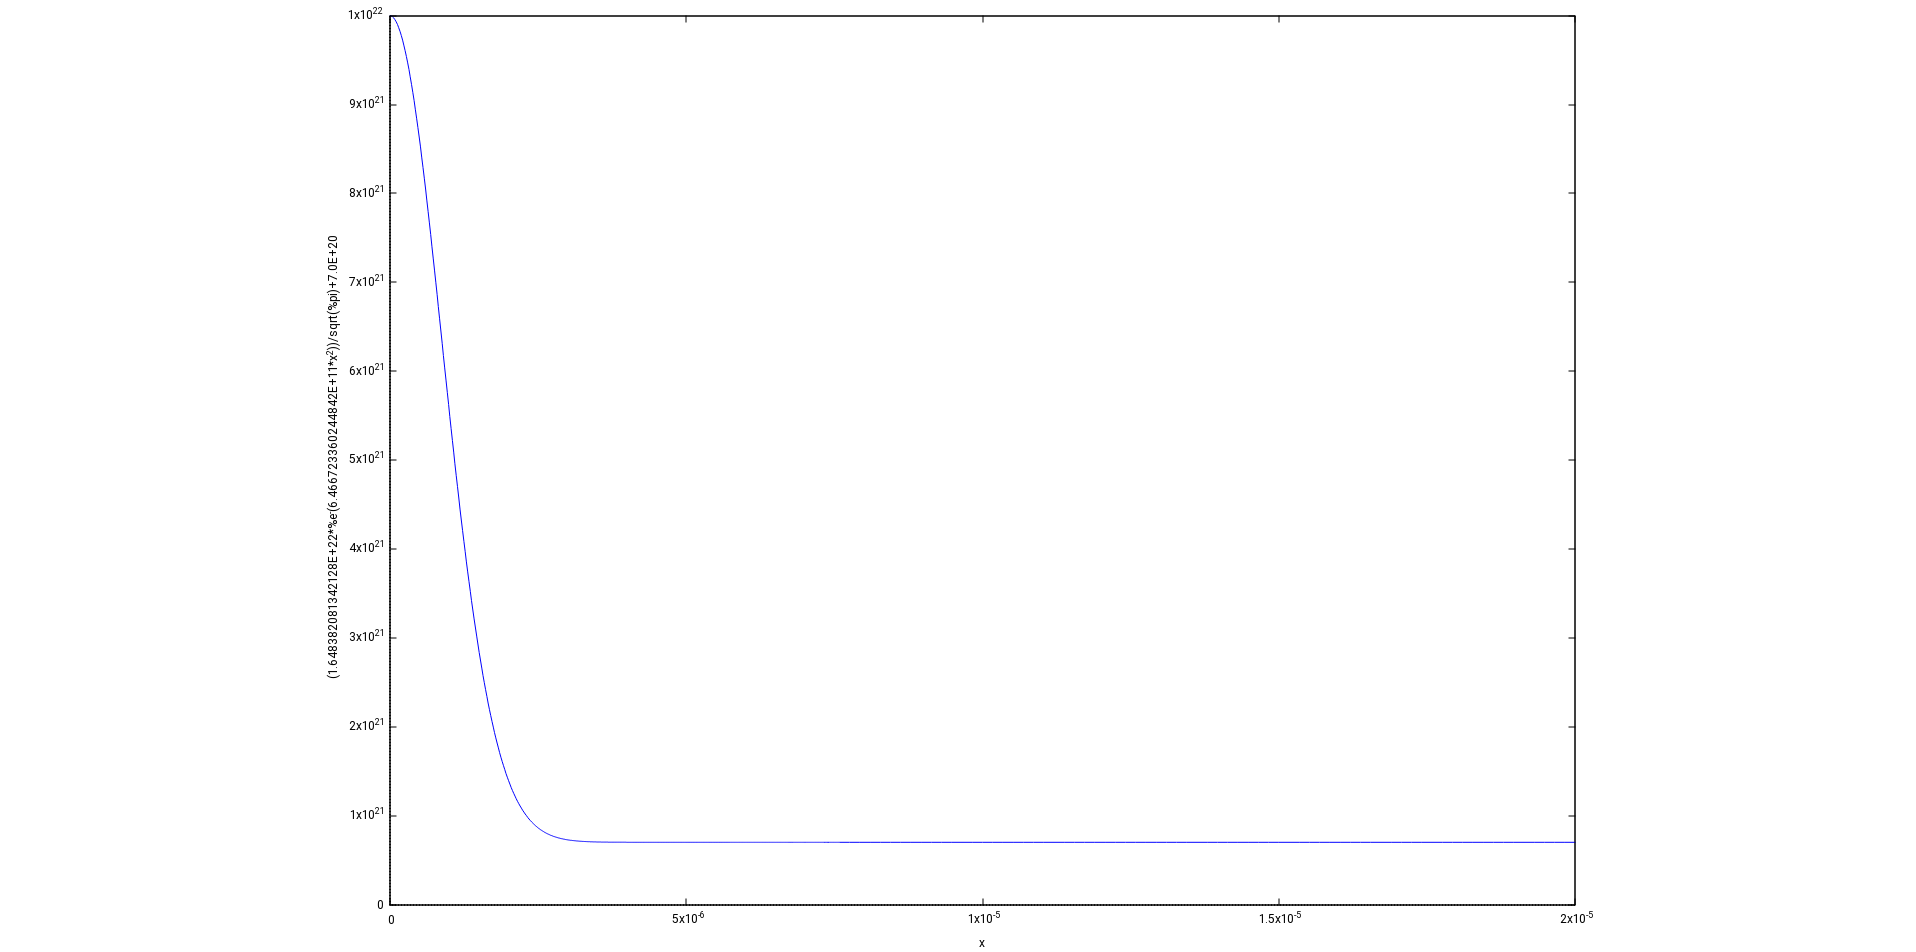
\includegraphics[width=0.75\textwidth]{p-well-diffusion.png}
	\caption{Dopant concentration after 3 hours}
	\label{pwell_drive_in_outcome}
\end{figure}

In \autoref{pwell_drive_in_outcome} we can see that after three hours we already have the desired even gradient which and deep penetration of dopants, which will give us a low $R_{DS}$.
\newpage
\subsection{PMOS threshold}
Now we take a look at the worst case of 4 stacked PMOS transistors, which is the highest stacking amount which will be possible in technologies relying on this process.
%%  ************    LibreSilicon's StdCellLibrary   *******************
%%
%%  Organisation:   Chipforge
%%                  Germany / European Union
%%
%%  Profile:        Chipforge focus on fine System-on-Chip Cores in
%%                  Verilog HDL Code which are easy understandable and
%%                  adjustable. For further information see
%%                          www.chipforge.org
%%                  there are projects from small cores up to PCBs, too.
%%
%%  File:           StdCellLib/Documents/LaTeX/schematic_OR4.tex
%%
%%  Purpose:        Schematic File for OR4
%%
%%  ************    LaTeX with circdia.sty package      ***************
%%
%%  ///////////////////////////////////////////////////////////////////
%%
%%  Copyright (c) 2018 by chipforge <hsank@nospam.chipforge.org>
%%  All rights reserved.
%%
%%      This Standard Cell Library is licensed under the Libre Silicon
%%      public license; you can redistribute it and/or modify it under
%%      the terms of the Libre Silicon public license as published by
%%      the Libre Silicon alliance, either version 1 of the License, or
%%      (at your option) any later version.
%%
%%      This design is distributed in the hope that it will be useful,
%%      but WITHOUT ANY WARRANTY; without even the implied warranty of
%%      MERCHANTABILITY or FITNESS FOR A PARTICULAR PURPOSE.
%%      See the Libre Silicon Public License for more details.
%%
%%  ///////////////////////////////////////////////////////////////////
    
    \begin{figure}[H] %\caption{Schematic}
       \centering
            \begin{circuitdiagram}{60}{33}
            \pin{2}{2.5}{L}{A}  % pin A, n-channel left
            \pin{2}{11.5}{L}{A}  % pin A, p-channel below
            \pin{2}{17.5}{L}{B}  % pin B, p-channel middle
            \pin{2}{23.5}{L}{C} % pin C, p-channel above
            \pin{2}{29.5}{L}{D} % pin D, p-channel above
            \pin{14}{2.5}{L}{B} % pin B, n-channel middle
            \pin{26}{2.5}{L}{C} % pin C, n-channel right
            \pin{38}{2.5}{L}{D} % pin D, n-channel right
            \trans{nenh*}{6}{4}{R}{}{}  % nmos left
            \trans{penh*}{6}{10}{R}{}{} % pmos below
            \trans{penh*}{6}{16}{R}{}{} % pmos middle
            \trans{penh*}{6}{22}{R}{}{} % pmos above
            \trans{penh*}{6}{28}{R}{}{} % pmos above
            \trans{nenh*}{18}{4}{R}{}{} % nmos middle
            \trans{nenh*}{30}{4}{R}{}{} % nmos right
            \trans{nenh*}{42}{4}{R}{}{} % nmos right
            \wire{8}{6}{8}{8}     % wire between nmos
            \ground{8}{0.5}{D}  % ground below nmos
            \power{8}{31.5}{U}{}  % power above left pmos
            \ground{20}{0.5}{D}  % ground below nmos
            \ground{32}{0.5}{D}  % ground below nmos
            \ground{44}{0.5}{D}  % ground below nmos
            \wire{8}{12}{8}{14}     % wire between nmos
            \wire{8}{18}{8}{20}     % wire between nmos and pmos
            \wire{20}{7}{20}{6}
            \wire{32}{7}{32}{6}
            \wire{8}{7}{51}{7}    % wire before inverter gates
            \wire{51}{2.5}{51}{11.5}  % wire on inverter gates
            \junct{8}{7}
            \junct{20}{7}
            \junct{32}{7}
            \junct{44}{7}
            \junct{51}{7}
            \trans{nenh*}{54}{4}{R}{}{} % nmos right
            \trans{penh*}{54}{10}{R}{}{} % pmos below
            \power{56}{13.5}{U}{}  % power above left pmos
            \ground{56}{0.5}{D}  % ground below nmos
            \wire{56}{7}{58}{7}    % wire before pin
            \wire{56}{6}{56}{8}    % wire before pin
            \junct{56}{7}
            \pin{59}{7}{R}{Z}  % pin Z
            \end{circuitdiagram}
            \caption{OR4 gate}
    \end{figure}

\newpage
\subsection{MOS gate verification}\label{gate_verify}
Now we have to verify that we don have relevant leakage on the gate with the thresholds and doping values we've set.

For that we use the formulas from \autoref{sub_threshold_leakage}

We can now plot multiple leakages for N- and P-channel transistors with a gate oxide thickness\footnote{See simulation/gate.wxmx} and with a surface concentration of $1e16\frac{1}{cm^3}=1e22\frac{1}{m^3}$ each
\begin{figure}[H]
	\centering
	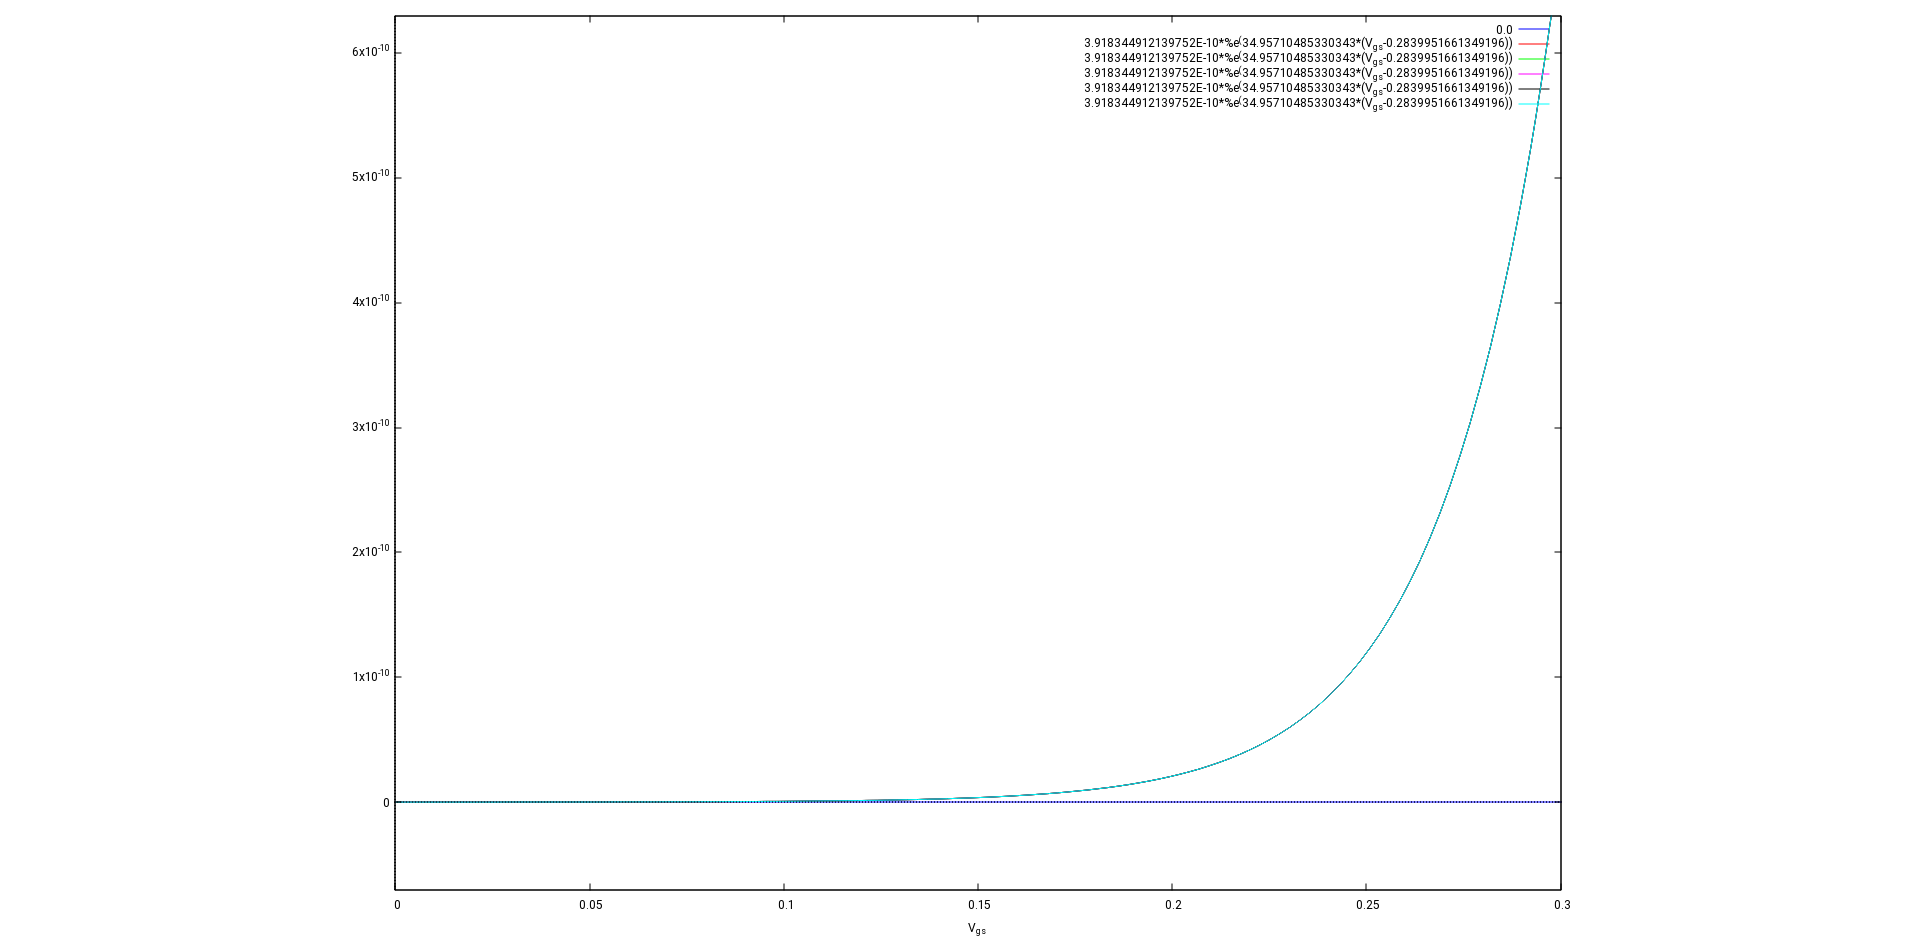
\includegraphics[width=\textwidth]{subthreshold_leagage.png}
	\caption{Subthreshold leakage plot(in Ampere)}
	\label{leagage_currents}
\end{figure}
In \autoref{leagage_currents} we see that with our gate oxide thickness this is really no problem, as we had expected.
From 0V up to 5V and further there is basically no leakage on the gate from the sub threshold current with $V_{Tn} \approx 0.39V$ and $V_{Tp} \approx -0.30V$.
That's good enough, as we will see in \autoref{nmos_dimensioning} and \autoref{pmos_dimensioning}.
There is actually a reduction of current when reaching the threshold because of the inversion of the capacity in the depletion zone\footnote{\url{https://people.eecs.berkeley.edu/~hu/Chenming-Hu_ch5.pdf}}, but I didn't include this into the calculation, because "TL;DR".
It's a TODO for release 2.1 of this process which will go sub $1 \mu m$
\newpage
\newcommand{\addAlignmentCross}[2]{
	\draw[line width=1.5mm, active,opacity=\OpacityLayout] (#1,#2+0.5) -- (#1+1,#2+0.5);
	\draw[line width=1.5mm, active,opacity=\OpacityLayout] (#1+0.5,#2) -- (#1+0.5,#2+1);
}

\section{Alignment strategy}
When having multiple layers exposed after each other, there is the problem on how to make sure that for instance vias are actually making contact with the below wire and the wire above.
For this purpose we have to align the masks, in order to avoid issues like shown in \autoref{what_can_go_wrong_with_alignment}

\begin{figure}[H]
	\centering
	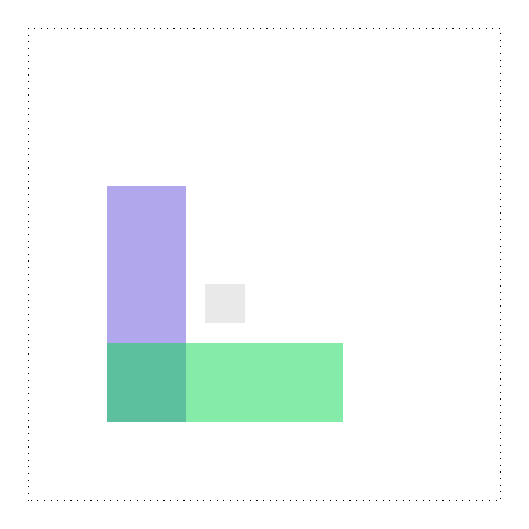
\begin{tikzpicture}
		\fill[metal1,opacity=\OpacityLayout] (1,1) rectangle (2,4);
		\fill[via1,opacity=\OpacityLayout] (2.25,2.25) rectangle (2.75,2.75);
		\fill[metal2,opacity=\OpacityLayout] (1,1) rectangle (4,2);
		\draw[dotted] (0.0,0) rectangle (6,6);
	\end{tikzpicture} 
	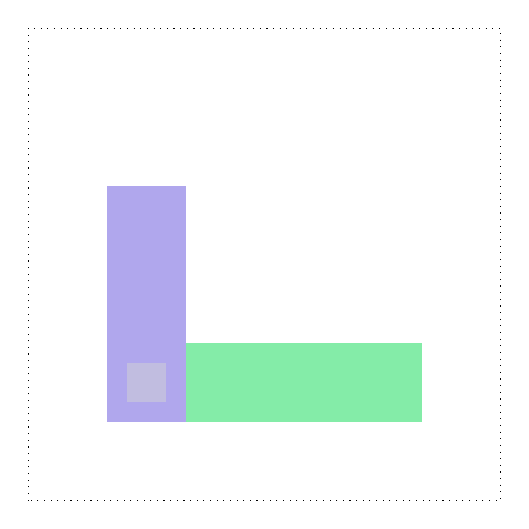
\begin{tikzpicture}
		\fill[metal1,opacity=\OpacityLayout] (1,1) rectangle (2,4);
		\fill[via1,opacity=\OpacityLayout] (1.25,1.25) rectangle (1.75,1.75);
		\fill[metal2,opacity=\OpacityLayout] (2,1) rectangle (5,2);
		\draw[dotted] (0.0,0) rectangle (6,6);
	\end{tikzpicture}
	\caption{What can go wrong with alignment}
	\label{what_can_go_wrong_with_alignment}
\end{figure}

In \autoref{what_can_go_wrong_with_alignment} we can see how the wires and vias are missing each other because of an exposure offset and the via is going nowhere in the best case and creates an (of course) undesired short circuit in the worst case. This has to be avoided by using alignment.

We have decided to use backside alignment because shining through the wafer from behind with infrared and finding an orientation marker isn't a problem with our simple CMOS process.\footnote{\url{https://patents.google.com/patent/US6376329}}

The stepper machine at HKUST\footnote{\url{http://www.nff.ust.hk/en/equipment-and-process/equipment-list/photolithography-module.html}} does that for us.

We need to add orientation cross hairs onto the layout edge in order to identify them during alignment

\begin{figure}[H]
	\centering
	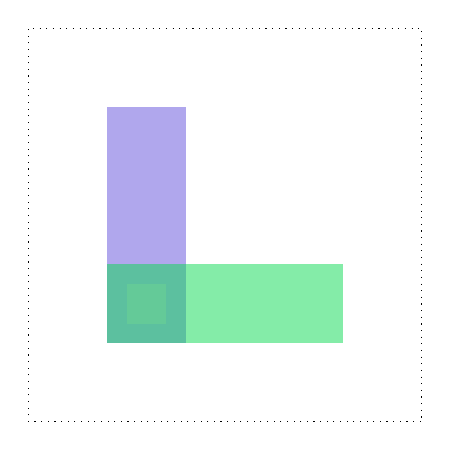
\begin{tikzpicture}
		\fill[metal1,opacity=\OpacityLayout] (1,1) rectangle (2,4);
		\fill[via1,opacity=\OpacityLayout] (1.25,1.25) rectangle (1.75,1.75);
		\fill[metal2,opacity=\OpacityLayout] (1,1) rectangle (4,2);
		\draw[dotted] (0.0,0) rectangle (5,5);
		% cross one
		\addAlignmentCross{0}{0}
		% cross two
		\addAlignmentCross{4}{4}
		% cross three
		\addAlignmentCross{4}{0}
		% cross four
		\addAlignmentCross{0}{4}
	\end{tikzpicture}
	\caption{Mask alignment with markers}
\end{figure}

Using the STI (active) mask for the cross hair structure is a good choice, because it's the lowest layer, will never be covered by any additional material and gives us a good contrast because it's silicon next to silicon dioxide.

\newpage

The "DRIE Etcher" can't etch more precise than $0.5 \mu m$ (Minimum Line/Space: $0.5 \mu m$) which means we will have to give the cross hair structure with the dimensions as shown in \autoref{cross_hair_dimensions}
\begin{figure}[H]
	\centering
	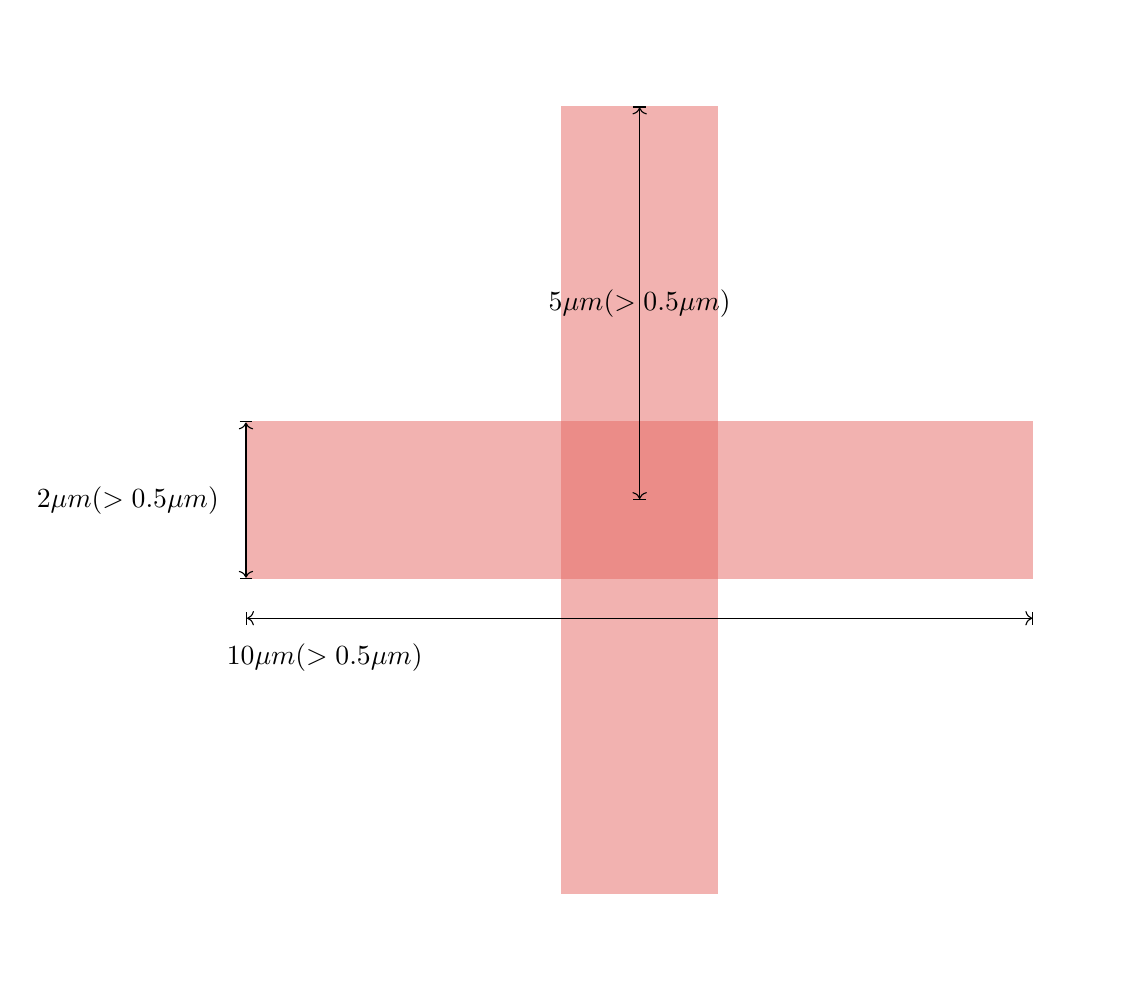
\begin{tikzpicture}
		\draw[line width=20mm, active,opacity=\OpacityLayout] (0,50mm) -- (100mm,50mm);
		\draw[line width=20mm, active,opacity=\OpacityLayout] (50mm,0) -- (50mm,100mm);
		\draw [|<->|] (0,4) -- (0,6); 
		\node at (-15mm,50mm) {$ 2 \mu m (> 0.5 \mu m) $};
		\draw [|<->|] (0,3.5) -- (10,3.5); 
		\node at (10mm,30mm) {$ 10 \mu m (> 0.5 \mu m) $};
		\draw [|<->|] (50mm,50mm) -- (50mm,100mm); 
		\node at (50mm,75mm) {$ 5 \mu m (> 0.5 \mu m) $};
	\end{tikzpicture}
	\caption{Cross hair dimension}
	\label{cross_hair_dimensions}
\end{figure}

We can now manufacture masks as shown in \autoref{mask_set_example} and align them using the infrared light from the stepper mask alignment and the provided electronic microscope.

\begin{figure}[H]
	\centering
	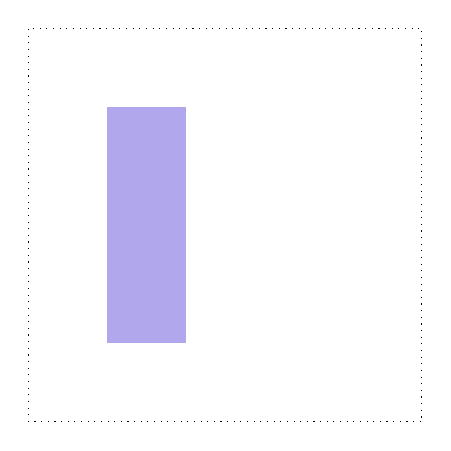
\begin{tikzpicture}
		\fill[metal1,opacity=\OpacityLayout] (1,1) rectangle (2,4);
		\draw[dotted] (0.0,0) rectangle (5,5);
		% cross one
		\addAlignmentCross{0}{0}
		% cross two
		\addAlignmentCross{4}{4}
		% cross three
		\addAlignmentCross{4}{0}
		% cross four
		\addAlignmentCross{0}{4}
	\end{tikzpicture} 
	\begin{tikzpicture}
		\fill[via1,opacity=\OpacityLayout] (1.25,1.25) rectangle (1.75,1.75);
		\draw[dotted] (0.0,0) rectangle (5,5);
		% cross one
		\addAlignmentCross{0}{0}
		% cross two
		\addAlignmentCross{4}{4}
		% cross three
		\addAlignmentCross{4}{0}
		% cross four
		\addAlignmentCross{0}{4}
	\end{tikzpicture} 
	
\begin{tikzpicture}
		\fill[metal2,opacity=\OpacityLayout] (1,1) rectangle (4,2);
		\draw[dotted] (0.0,0) rectangle (5,5);
		% cross one
		\addAlignmentCross{0}{0}
		% cross two
		\addAlignmentCross{4}{4}
		% cross three
		\addAlignmentCross{4}{0}
		% cross four
		\addAlignmentCross{0}{4}
	\end{tikzpicture}
	\caption{Layout masks with alignment markers}
	\label{mask_set_example}
\end{figure}
\newpage
\section{Simulation with parameters}
\end{document}
